\section{Vlastní řešení}
Tato sekce se věnuje definici požadavků na vlastní řešení a výběru vhodných technologií.

\subsection{Záměr}
Vytvoření otevřené IoT platformy, která bude určena pro nejrůznější elektrotechnické kutily a technické nadšence. K dispozici bude zdarma veřejná instance sloužící primárně pro uživatele, kteří si chtějí platformu jednoduše a rychle vyzkoušet a nebo chtějí provozovat pouze pár zařízení. Pro ty, kteří chtějí mít plnou kontrolu nad svými daty a být nezávislí na připojení k internetu, bude k dispozici možnost hostingu celého řešení na vlastním hardwaru. K platformě půjde připojit různorodá zařízení a bude vytvořeno schéma, pomocí kterého zařízení popíší platformě vlastní funkčnost/schopnosti. Na základě těchto informací se automaticky uživateli vygeneruje webové rozhraní ke sledování a ovládání jeho zařízení.

Na bezpečnost bude kladen vysoký důraz. Primárně bude založena na uživatelských účtech, které budou mít oprávnění pouze ke svým zařízením, případně těm, ke kterým dostali oprávnění od jiných uživatelů. Každý uživatel by měl mít k dispozici vlastní izolované prostředí, v rámci kterého budou jeho zařízení komunikovat. Uživateli bude umožněno sledovat všechny zprávy posílané mezi jeho zařízeními a platformou.


\subsection{Popis domény}
Tato kapitola obsahuje popis jednotlivých entit, se kterými platforma pracuje.
\begin{figure}[htbp]
    \centering
    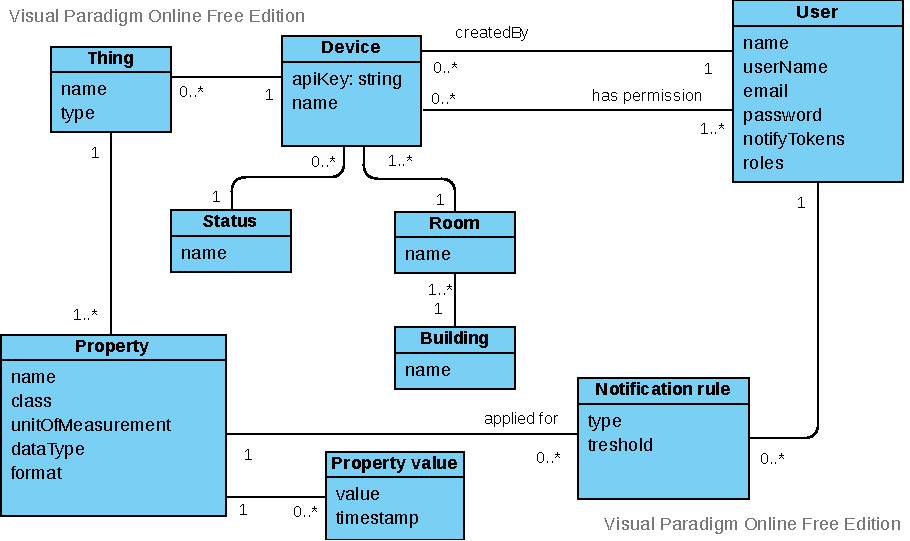
\includegraphics[width=\textwidth]{img/domain.pdf}
    \caption{  \label{domain-model}Doménový model}
\end{figure}
\begin{itemize}
    \item \textbf{Uživatel (User)} - osoba, která interaguje s webovým rozhraním.
    \item \textbf{Zařízení (Device)} - fyzické zařízení, které komunikuje s platformou a dále se dělí na věci.
    \item \textbf{Stav (Status)} - v jakém stavu se zařízení nachází (např. odpojeno).
    \item \textbf{Věc (Thing)} - logické uskupení vlastností, např. meteostanice.
    \item \textbf{Vlastnost (Property)} - určitá veličina, jejíž hodnota se odesílá na platformu (např. teplota), která případně umožňuje být platformou nastavena.
    \item \textbf{Hodnota vlastnosti} - hodnota v určitém časovém okamžiku.
    \item \textbf{Budova (Building)} - místo, které se dále dělí na místnosti.
    \item \textbf{Místnost (Room)} - uskupení více zařízení.
    \item \textbf{Notifikační pravidlo} - za jaké podmínky se má uživateli odeslat notifikace.
\end{itemize}


\subsection{Případy užití}
Tato kapitola popisuje identifikované případy užití, které současně slouží jako podklad funkčních požadavků kladených na řešení. Figurují v nich následující aktéři:
\begin{itemize}
    \item Neautorizovaný uživatel - představuje nepřihlášeného uživatele webového rozhraní
    \item Uživatel - přihlášený uživatel webového rozhraní
    \item Administrátor - autentizovaný uživatele s vyšším stupněm oprávnění
    \item Zařízení - koncové zařízení komunikující s platformou
\end{itemize}

\begin{figure}[htbp]
    \centering
    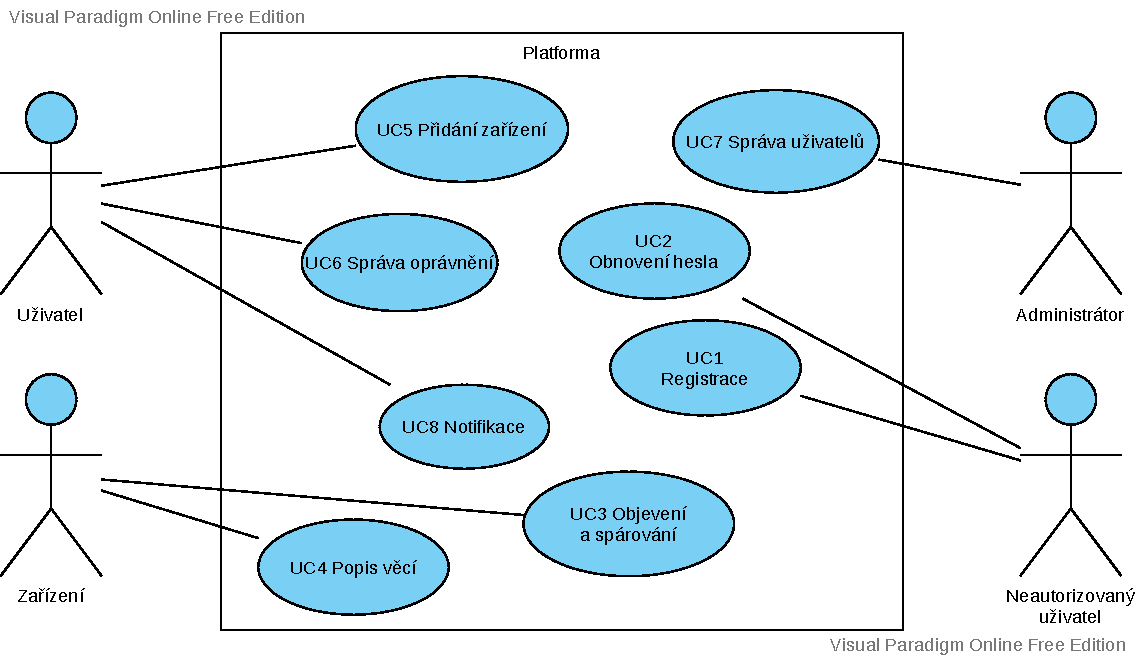
\includegraphics[width=0.9\textwidth]{img/use_case.pdf}
    \caption{Případy užití}
\end{figure}

\paragraph{UC1 Registrace uživatele}
Neautentizovaný uživatel vyplní registrační formulář obsahující jméno, přijmení, uživatelské jméno, heslo a email. Při zpracování požadavku na serveru bude zajištěna unikátnost uživatelského jména a emailu napříč databází. Uživatel bude informován o úspěchu/neúspěchu akce. Po úspěšné registraci bude automaticky přihlášen, pokud nezrušil ve formuláři zaškrtávátko \uv{Automaticky přihlásit}. Následně mu bude odeslán uvítací email na zadanou emailovou adresu.

\paragraph{UC2 Obnovení hesla}
Součástí přihlašovacího formuláře bude odkaz na stránku pro obnovení zapomenutého hesla, kde bude uživatel dotázán na emailovou adresu, kterou použil při registraci. Po zadání, pokud daná emailová adresa je součástí některého uživatelské účtu, bude odeslán email s odkazem pro obnovu hesla. Na tomto odkazu bude uživatel vyzván k zadání hesla nového.

\paragraph{UC3 Objevení a spárování nového zařízení}
Zařízení, pokud ještě není spárované s platformou, po zapnutí vyzve uživatele k zadání svého uživ. jména k platformě. Toto zadání bude umožněno vytvořením Wifi přístupového bodu, na kterém poběží kaptivní portál - po připojení telefonem/počítačem se automaticky zobrazí webová stránka s formulářem pro zadání údajů. Následně se zařízení připojí k platformě, ohlásí jaké má věci, popíše jejich vlastnosti a bude ji informovat, kterému uživateli (podle zadaného uživ. jména) má zobrazit možnost přidání nového zařízení. Pokud si uživatel dané zařízení přidá (viz. \hyperref[UC5]{UC5}), platforma následně odešle zařízení API klíč, které si ho uloží a přihlásí se pomocí toho klíče k platformě (nyní je spárované).

\paragraph{UC4 Popis věcí}
Zařízení při ohlašování definice věcí a jejich vlastností musí oznámit mimo jiné typ věci. Platforma bude podporovat kromně generického (generic) typu další 3 typy věcí, pro které bude speciální zobrazení v uživatelském rozhraní:
\begin{itemize}
    \item \textbf{Switch} - přepínač, který se nachází ve stavu on/off. V rozhraní bude věc reprezentována dvoustavovým přepínačem, který při kliknutí odešle změnu o stavu na druhý, než ve kterém se aktuálně nachází. (využití např. vypínač světla)
    \item \textbf{Activator} - spínač, který má pouze jeden stav. V rozhraní bude věc reprezentována tlačítkem, které na stisk odešle aktivaci zařízení. (využití např. ovladač pojízdné brány)
    \item \textbf{Sensor} - v rozhraní bude reprezentován jako widget zobrazující aktuální hodnotu první vlastnosti. Po rozkliknutí se zobrazí graf vizualizující průběh hodnoty v čase za posledních 24h.
    \item \textbf{Generic} - obecný typ, u kterého zařízení popíše strukturu, datové typy a názvy příslušných vlastností. V uživatelském rozhraní bude věc reprezentována jako Widget, který po kliknutí zobrazí Dialogové okno umožňující zobrazení a ovládání všech vlastností dle konfigurace.
\end{itemize}

\paragraph{UC5 Přidání zařízení}
\label{UC5}
Uživateli na stránce \uv{Správa zařízení}, v případě že bude detekováno nové zařízení, v sekci \textit{Přidat zařízení} se zobrazí (bez nutnosti aktualizace stránky) možnost přidat nové zařízení. Při kliknutí na tlačítko přidat se zobrazí jednoduchý formulář pro zadání umístění a názvu zařízení - bude předvyplněn název, který ohlásilo zařízení. Uživatel formulář potvrdí, systém následně vytvoří dané zařízení, přidá uživateli k němu oprávnění a na stránce \uv{Ovládání} už bude uživatel moci sledovat aktuální stav věcí a případně je i ovládat (pokud to umožňují).

\paragraph{UC6 Správa oprávnění}
Uživatel na stránce \uv{Správa zařízení} v sekci \textit{Správa} bude mít zobrazena všechna zařízení, ke kterým má uživatel oprávnění. Rozhraní umožní pro každé zařízení, ke kterému má příslušné oprávnění pro správu, jeho smazání a pomocí formuláře editaci - názvu, umístění a změnu oprávnění pro jednotlivé uživatele. Tyto oprávnění budou rozděleny na tři úrovně:
\begin{itemize}
    \item Čtení - uživatel může zobrazit veškeré údaje o zařízení.
    \item Ovládání - uživatel může zařízení ovládat.
    \item Správa - uživatel může editovat veškeré informace o zařízení (včetně oprávnění).
\end{itemize}

\paragraph{UC7 Správa uživatelů}
Administrátor má k dispozici stránku \uv{Správa uživatelů}, kde se mu zobrazí seznam všech registrovaných uživatelů. Jednotlivé uživatele může smazat a pomocí formuláře editovat všechny jejich osobní údaje a změnit heslo pro přihlášení.

\paragraph{UC8 Notifikace}
Rozhraní umožní uživateli nastavit pravidlo pro libovolnou věc, při kterém se odešle Web Push notifikaci (technologie umožňující serveru odeslat upozornění do prohlížeče klienta \cite{web-push}) na jeho zařízení. Pro nastavení bude zobrazený formulář umožňující výběr z vlastností dané věci, po vybrání se zobrazí výběr akce, při jejímž splnění chce uživatel obdržet notifikaci (překročení hodnoty / vždy / hodnota bude rovna) a případné pole pro zadání limitní hodnoty. Dále půjde zobrazit rozšířené nastavení pro konkrétní notifikační pravidlo umožňující nastavení času a konkrétních dnů v týdnu, kdy bude pravidlo platné (ve výchozím stavu bude vždy). Těchto pravidel si bude moci nastavit libovolný počet pro každé zařízení, ke kterému má oprávnění pro čtení.



\subsection{Nefunkční požadavky}

\paragraph{N1 Řešení spustinelné na Linux systému}
Systém bude možno provozovat na Linuxovém serveru (Debian) a také na platformě Raspberry Pi (verze 3B+/4, OS Raspbian).

\paragraph{N2 Responzivní webové rozhraní}
Aplikace bude nabízet responzivní webové rozhraní přizpůsobené pro zobrazení na mobilních zařízeních i stolních počítačích. Uživatelské rozhraní bude kompatibilní s prohlížeči Mozilla Firefox verze 80, Chrome verze 80 a Safari na iOS. Dále bude implementovat tzv. PWA (Progresivní webová aplikace) - bude využívat cache pro statické soubory pro rychlé načítání, spustitelné offline a na zařízení Android půjde v aplikaci chrome přidat na plochu a následně vypadat jako nativní aplikace.

\paragraph{N3 Rozhraní realizováno jako SPA}
Single page application (SPA) je webová aplikace, která utilizuje JavaScript tak, aby při interakci v rámci aplikace se nemusela načítat celá stránka, ale pouze chytře překresluje potřebné části. Výsledkem je mnohem přijemnější uživatelský zážitek, než při čekání na stažení a překreslení celé stránka po kliknutí na odkaz.

\paragraph{N4 Validace}
Uživatel v průběhu vyplňování formulářů v rozhraní obdrží interaktivní zpětnou vazbu v případě zadání nevalidních údajů. Interaktivní zpětnou vazbou jsou myšleny následující scénáře při průchodu formuláře:
\begin{itemize}
    \item Zadání nové hodnoty a opuštění pole - bude provedena validace a v případě nevalidního vstupu, bude uživatel vizuálně  upozorněn.
    \item Editace již zadané hodnoty v poli - validace bude provedena po každé změně (stisknutí klávesy), uživatel bude vizuálně upozorněn v případě nevalidního vstupu.
\end{itemize}

\paragraph{N5 Koncová zařízení}
Bude specifikován protokol, pomocí kterého s platformou budou zařízení komunikovat včetně definování schématu komunikace. Platforma umožní připojení libovolného zařízení, pokud použije definovaný protokol a bude se řídit schématem pro komunikaci.

\paragraph{N6 Výkonnostní požadavky}
Systém bude stabilní a zvládne obsluhovat stovku zařízení, kde každé bude odesílat změnu stavu s periodicitou 30 vteřin. Při tomto dlouhodobém zatížení nebude docházet k pádům systému ani k výraznému zpoždění komunikace (RESTful požadavky pod 500 ms).

\paragraph{N7 Konfigurace systému}
Veškerá konfigurace týkající se externích služeb jako jméno a heslo do databáze, číslo portu pro komunikaci atd. bude konfigurovatelné pomocí promněných prostředí (env variables). Detailní popis proměnných bude obsažen v instalační příručce.


\subsection{Vybrané technologie}
Tato sekce se věnuje výběru protokolu pro komunikaci se zařízeními a programovacího jazyka, ve kterém bude řešení implementováno včetně výběru příslušných knihoven.

\subsubsection{Komunikační protokol}
Komunikačních protokolů je velké množství a jeho výběr přímo závisí na použitém přenosovém médiu. Při použití specializovaných sítí jako LoRa nebo Zigbee, nemáme moc velkou flexibilitu ve výběru. Zařízení podporující tyto specializované sítě jsou poměrně drahá, ale umožňují běh na baterii. Zatímco využití Wifi sítě nám dává obrovskou flexibilitu ve výběru protokolů a zařízení podporující připojení k Wifi nebyly nikdy více cenově dostupné jako dnes. Primárně z finančních nároků a možnosti využití stávající Wifi infrastruktury v domácnosti jsem se rozhodl pro Wifi jako bezdrátové médium. Současně díky přímé podpoře IP protokolu nebudu muset vytvářet bridge mezi serverem a sítí se zařízeními jako např. při použití Bluetooth či LoRa.

Z protokolů pro komunikaci je dnes nejpoužívanější HTTP, který ale nativně nepodporuje obousměrnou komunikaci, kdy zařízení může poslat zprávu serveru a stejně tak server zprávu zařízení, kterou pro ovládání zařízení budu potřebovat. Z obousměrných protokolů se velmi osvědčil WebSocket, který lze velmi snadno kombinovat s HTTP. Jedná se o protokol postavený nad TCP, který naváže spojení a obě strany mohou posílat zprávy \cite{websocket}. Je to velmi pěkné řešení pro posílání zpráv, ale neumožňuje nativně systematickou filtraci nebo odběr pouze určitých zpráv a nepočítá s během na nespolehlivých zařízeních. Proto přímo pro IoT vznikl otevřený síťový protokol MQTT, kterým jsem si zvolil jako komunikační protokol, jehož specifikaci vydává nezisková organizace \textit{OASIS}. Využívá asynchronní vzor \textit{publish-subsribe} (v podstatě rozděluje akci na dvě události - vytvoření akce a její obsluhu) a byl speciálně navržen pro potřeby běhu na jednoduchých embeded zařízení s minimálním datovým tokem. Podrobný přehled všech protokolů využívaný pro IoT viz. \cite{protocols}.

\begin{figure}[htbp]
    \centering
    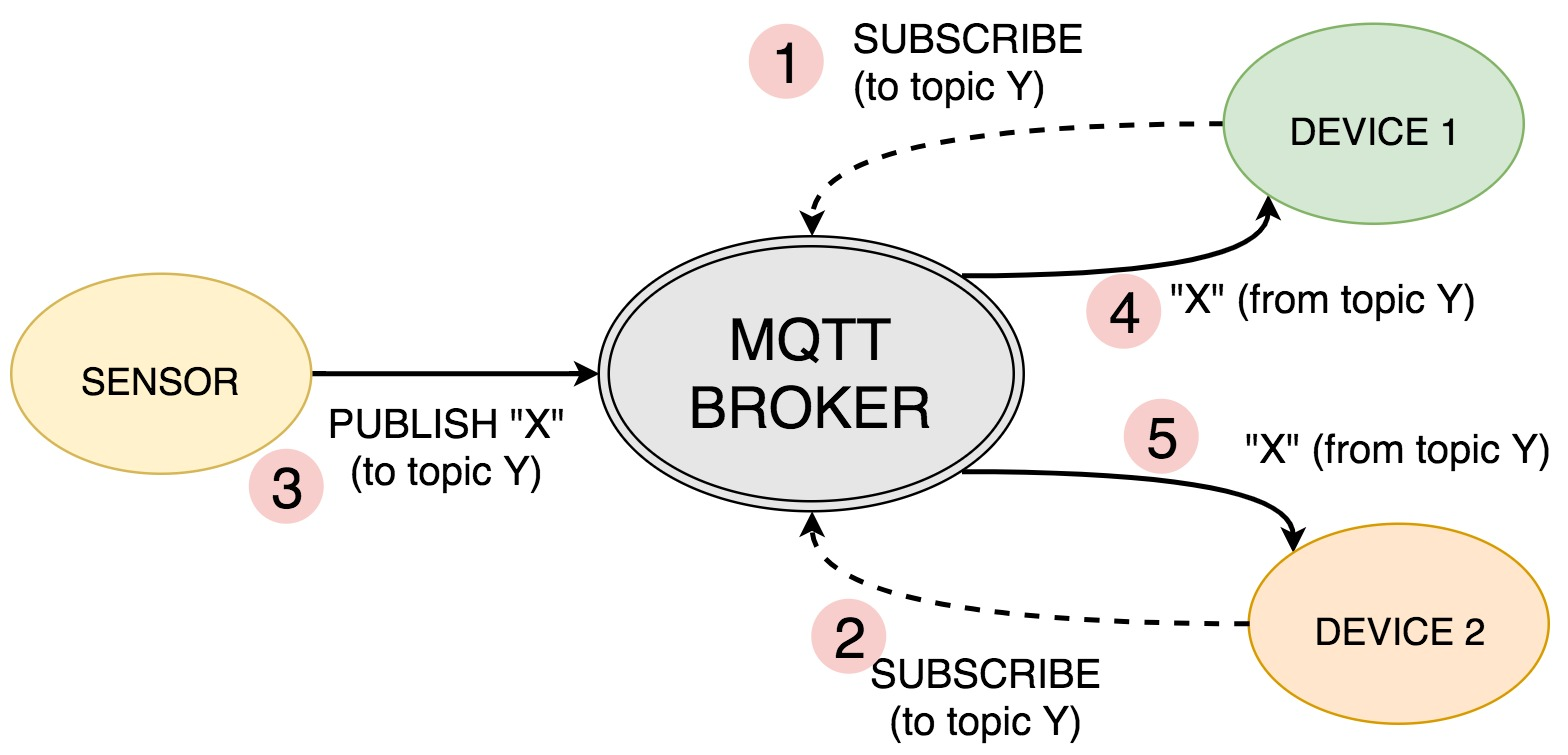
\includegraphics[width=0.7\textwidth]{img/mqtt-communication.jpeg}
    \caption{Ukázka komunikace MQTT \cite{img-mqtt-communication}}
\end{figure}

\label{mqtt-description}
MQTT se vyvíjí již od roku 1999 a momentálně nejpoužívanější verzí je 3.1.1, pro kterou vznikla specifikace v roce 2014. Protokol primárně běží nad TCP/IP, ale lze využít v jakékoliv síti, kde je zaručeno správné pořadí dat, beztrátovost a obousměrnost komunikace. Protokol definuje 2 typy entit: \uv{MQTT broker} a \uv{klient}. MQTT broker je server, který přijímá všechny zprávy od připojených klientů a přeposílá je příjemncům (klientům). MQTT klient je jakékoliv zařízení (od embeded až po server), které komunikuje s brokerem přes síť. \cite{mqtt}

Posílaná data jsou hierarchicky rozdělena do tzv. témat. Téma je textový řetězec o maximální délce 65\,536\,Bytů s oddělovačem lomítko (ukázka \uv{house/bedroom/light}). Pokud klient chce odeslat (publish) data, tak pošle zprávu brokeru s daty a tématem, do kterého zpráva patří. Broker potom zprávu odešle všem klientům, kteří jsou přihlášeni k odběru (subscribe) z daného tématu. O odběr se klient musí přihlásit a to buď přímo specifikuje plný název topicu nebo částečný s použitím zástupných znaků. MQTT počítá s případnou nespolehlivostí koncových zařízení či sítě, a proto umožňuje klientovi při přihlášení definovat \uv{Last Will and Testament} (\hypertarget{LWT}{LWT}). Při přihlášení klient oznámí téma a zprávu, která se odešle v případě nesprávně odpojeného klienta (výpadek sítě / chyba zařízení). Takto lze notifikovat ostatní zařízení, že došlo ke ztráně spojení s daným klientem. \cite{mqtt}

Broker podporuje 3 třídy QoS (Quality of service), kterou lze specifikovat pro každou zprávu jednotlivě v závisloti na její důležitosti. Seřazeny jsou vzestupně dle náročnosti na systém (overhead) \cite{mqtt}:
\begin{itemize}
    \item \textbf{0 - Maximálně jednou} - zpráva je odeslána pouze jednou a klient ani broker nijak nepotvrzují její přjetí
    \item \textbf{1 - Alespoň jednou} - zpráva je odeslaná několikanásobně, dokud není potvrzené její přijetí
    \item \textbf{2 - Právě jednou} - odesílatel a příjemce navazují dvoucestný hand-shake, aby bylo zaručeno přijmutí zprávy právě jednou
\end{itemize}


\subsubsection{Programovací jazyk}
Programovacích jazyků jsou dnes na trhu stovky a každý má své specifické pozitivní i negativní vlastnosti. Při výběru je tedy vždy potřeba zohlednit jeho přínos pro použití na daném projektu. Kromě jazyka samotného je příhodné analyzovat dostupné knihovny a frameworky, které lze v projektu použít a značně tak urychlit celkový vývoj. Pro implementaci této práce byl zvolen jazyk JavaScript konkrétně jeho nadmnožina TypeScript a to z několika důvodů.

Vzhledem k povaze zvoleného protokolu pro komunikaci se zařízeními, jenž je založený na asynchronních zprávách, je JavaScript velmi vhodný, protože je založený na asynchronní event-driven \cite{nodejs} architektuře. Tato architektura nabízí velice elegantní přístup pro zpracování akcí, kde se musí čekat na výsledek jako např. u síťové komunikace či právě asynchronních zpráv. V tradičním jazyce jako Java nebo C++ se toto čekání musí řešit pracným vytvořením nového vlákna, které čeká na výsledek a následným zpracováním. V NodeJS je programátor od této problematiky odstíněn a může se tak plně věnovat tvorbě aplikační logiky, aniž by měl znalosti a zkušenosti s vícevláknovým programováním.

JavaScript je jediný programovací jazyk, který umožňuje psaní jak serverových aplikací, tak i uživatelského rozhraní formou webové stránky a jeho přímé vykonávání ve webovém prohlížeči klienta. Využití jednotného jazyka pro vývoj serveru i uživ. rozhraní přináší obrovskou výhodu v podobě možnosti sdílet nejenom definice pro objekty, ale i přímo části kódu. Toto je velmi vhodné například pro jednotné validace formulářů, různé datové transformace a sdílení aplikační logiky pro frontend \uv{optimistické aktualizace} (aktuální trend, nečekat na potvrzení požadavku ze serveru, ale rozhraní aktualizovat, jako by požadavek byl úspěšný a pouze v případě neúspěchu zobrazit stav ze serveru). Dále jednotný jazyk umožňuje programátorům při vývoji v případě potřeby pohodlně pracovat na obou částech aplikace, aniž by se museli učit nový jazyk.

\paragraph{TypeScript} Je nadmnožina JavaScriptu, která navíc přidává komplexní typový systém \cite{ts} a rozhodl jsem se ho využít jako hlavní programovací jazyk jak pro backend tak i frontend. Jedná se o OpenSource jazyk vyvíjený společností Microsoft, který jeho vznikem chtěl usnadnit přechod C\# a .NET vývojářům k webovým aplikacím \cite{ts}. Mnoho lidí z JavaScript komunity považuje TypeScript jako kontroverzní počin, protože přidává složitost k velmi elegantnímu jazyku a zvyšuje časovou náročnost vývoje. Já jsem dlouhou dobu tento názor také zastával, ale v posledních letech při práci na větších projektech a díky zkušeností z jiných jazyků (včetně striktně typových jako C++ a Java), jsem změnil svůj názor ve prospěch TypeScriptu. Souhlasím, že na první pohled prodlužuje dobu vývoje. Programátor musí psát věci navíc oproti čistému JavaScriptu, ale v dlouhodobém životním cyklu projektů se tato práce \uv{na víc} mnohonásobně vrátí. A to v podobě statické kontroly typů, která minimalizuje riziko pádu aplikace a umožňuje  lepší statickou analýzu kódu, a dále jako největší přínos pro mne jako programátora TypeScript přináší funkční \uv{našeptávání} ve vývojovém prostředí, které pro JavaScriptu i přes veškeré snahy bohužel funguje ve velmi omezené míře.

\subsubsection{Server}
Pro běh JavaScript na straně serveru existuje několik prostředí např. SpiderMonkey, NodeJS či Rhino. Pro realizaci bylo zvoleno prostředí NodeJS, které má pravděpodobně aktuálně největší a nejaktivější komunitu ze všech serverových prostředí pro běh aplikací napříč programovacími jazyky. Pro správu knihoven používá balíčkovací systém npm (jsou i jiné alternativy), ze kterého se stal největší ekosystém na světě, který je zastřešený neziskovou společností \uv{npm, Inc.} provozující centrální repozitář se všemi dostupnými moduly pro NodeJS. Díky sve centralizaci je velmi jednoduchý na používání, ale v posledních letech, kdy se JavaScript zpopularizoval a nyní je jedním z nejoblíbenějších jazyků \cite{survey-languages}, ukázala se centralizace jako poměrně nešťastné řešení kvůli vysokým nákladům na provoz infrastruktury. Pro představu velikosti ekosystému: npm v roce 2020 obsahoval 1\~200\~000 modulů a druhý největší systém RubyGems \uv{pouhých} 350\~000 \cite{modulecounts}. Všechny moduly jsou k dispozici zcela zdarma a díky takto aktivní komunitě lidí, kteří dávají k dispozici své knihovny ostatním, je vysoce pravděpodobné, že pokud chceme řešit nějaký problém, tak na něj již existuje knihovna.

\paragraph{ExpressJS}\label{expressjs} Platforma bude implementovat RESTful webové rozhraní a pro jeho implementaci byl zvolen minimalistický framework ExpressJS. První jeho verze vznikla již v roce 2010 a dodnes je mezi vývojáři velmi oblíbený a v mnohém ovlivnil směr vývoje většiny frameworků. Jeho největší výhoda je vysoká flexibilita. Nabízí pouze základní definici způsobu pracování s HTTP požadavky a možnost registrovat tzv. middleware - software, který rozšiřuje funkcionalitu. Veškerá funkcionalita je dodávána pomocí middlewarů, které jsou k dispozici jako moduly. Vývojář si tedy může výsledný server poskládat přesně dle svých představ, kterých existují desítky, vytvořených přímo od autorů a další stovky od komunity. \cite{expressjs}


\paragraph{AgendaJS} Knihovna pro perzistentní plánování úkolů pro NodeJS \cite{agendajs}. Umožňuje zpracování/plánování/perzistenci úkolů a jejich opětovné spouštění v případě chyby \cite{agendajs}. Tato knihovna bude primárně využita pro zajištění odeslání emailů a pro spouštění případných plánovaných akcí. Proč v souvislosti s odesláním emailů? Jejich zpracování je závislé na třetí straně - emailovém serveru, který nemusí být vždy dostupný. Pokud systém bude mět odeslat email, tak tímto způsobem bude zajištěno, že i v případě selhání bude email opětovně odeslán, jakmile to bude možné.

\paragraph{Socket.IO}\label{socketio} Pro zajištění aktualizace rozhraní v reálném čase bude využita knihovna SocketIO umožnující navázání obousměrného spojení pro real-time komunikaci. Jedná se o velice populární a časem ověřené řešení, které zajišťuje kompatibilitu i s prohlížeči nepodporujícími moderní technologii WebSocket.


\subsubsection{Uživatelské rozhraní}
Prvním bezesporu světoznámým průkopníkem ve světě JavaScriptu pro tvorbu uživatelského rozhraní byla knihovna \textit{jQuery}, která existuje dodnes, ale spíše se již považuje za přežitek doby. Dnes existuje obrovské množství Frameworků a knihoven pro tvorbu frontendu, ať pro tvorbu na straně serveru nebo přímo na straně uživatele v prohlížeči. Trend dnešní doby je přesouvat generování rozhraní na stranu uživatele, jak kvůli snížení výkonnostních nároků na server, tak spíše kvůli lepší odezvě a uživatelskému zážitku. Mezi nejznámější JavaScriptové frameworky patří bezpochyby Angular, Vue.js, Svelte a nesmím zapomenout na React, který je sice knihovna, ale řadí se na stejnou úroveň. Já jsem si zvolil jako hlavní prostředek pro tvorbu rozhraní React právě proto, že se jedná o knihovnu. Framework se vyznačuje tím, že vynucuje určité problémy řešit jistým způsobem bez možnosti volby. Má to své výhody a nevýhody a do větších týmů bych rozhodně volil raději framework. Tento projekt ale budu vytvářet primárně sám a mám velice rád flexibilitu a možnost volby. V začátcích to bývá časově náročnější, ale vidím v tom obrovskou možnost osobního růstu, protože při každé volbě musím hodnotit výhody/nevýhody a nakonec retrospektivně vidím následky svých rozhodnutí. Mimo to za vývojem Reactu stojí Facebook a je používán největšími technologickými spočnostmi světa (Yahoo!, Nextflix a Airbnb \cite{react-companies}), takže je jistá jeho dlouhodobá podpora a od roku 2013, kdy byla vydána první verze, je dobře odladěný a ověřený.

\paragraph{React} Je deklarativní, efektivní a flexibilní knihovna pro tvorbu rozhraní. Kód dělí do malých izolovaných částí kódu nazvaných \uv{komponenty}, které se skládají do sebe a mohou tvořit komplexní uživatelská rozhraní. Pro vysoký výkon využívá techniku virtuálního DOM - nejprve si vytvoří virtuální strom podoby rozhraní v paměti, který následně porovná s aktuální podobou vykreslenou v prohlížeči a zmanipuluje pouze ty části, které se od posledního vykreslení změnily. Díky tomu je velice efektivní a dokáže vykreslovat komplexní stránky s obrovským množstvím dat. \cite{react}